% !TEX = root../thesis.tex

\chapter{Search for a Long Lived Scalar Boson}
\section{Introduction} \label{sec:ana_intro}
This chapter describes the search for beyond the standard model (BSM) particles using data taken by the CMS detector from 2016-2018. The following sections outline the choice of datasets and simulated samples, event selection criteria, methods of background estimation and statistical analysis for signal extraction, and results.

\section{Data and Simulated Samples} \label{sec:ana_samples}

\subsection{Data Samples} \label{sec:ana_data}
As discussed in chapter~\ref{chap:exp}, events that pass at least 1 HLT path are stored for future analysis. These events are collected and sorted into datasets based on the number, flavor, and type of physics objects used in the HLT path. It can be noted that these datasets are not disjoint; one event can be sorted into multiple datasets if it satisfies more than a single HLT path. The data is maintained and updated by the Physics Data and Monte Carlo Validation (PdmV) group, which also provides recommendations on optimal usage for physics analysis~\cite{pdmv}. This search utilizes the PdmV recommended datasets for Run-2 analyses, referred to as Ultra-Legacy (UL), which has been reprocessed using the most current calibration for detector responses and alignment. Although the characteristic signature of this analysis is two displaced photons, the HLT double photon triggers present in Run-2 are unsuitable for the phase space of signal photons. Therefore we utilize the leptonic decay of the associated \VZ which provides a robust trigger. Since we are interested in \VZ decays to either electrons or muons, we use the datasets labeled as SingleMuon or SingleElectron (renamed to EGamma in 2018).

The reprocessed datasets must be cross referenced with the "Golden JSON": a certificate created by the Data Quality Monitoring (DQM) group within CMS by monitoring each sub-detector system in order to veto collisions that occur during sub-optimal conditions. The total integrated luminosity recorded by CMS during Run-2 was $164\unit{fb^{-1}}$; however, only $138\unit{fb^{-1}}$ of that was certified for analysis. The total integrated luminosity and uncertainty per year for collisions recommended by DQM can be seen in table~\ref{tab:intLumi}.

\begin{table}[h]
	\centering
	\caption[Table of integrated luminosity per year~\cite{cmslumi2016,cmslumi2017,cmslumi2018}.]{Table of integrated luminosity per year~\cite{cmslumi2016,cmslumi2017,cmslumi2018}.}
	\label{tab:intLumi}
	\begin{tabular}{l|l|l|l|l}\hline
		Year & 2016 & 2017 & 2018 & 2016-2018\\
		\hline
		\hline
		Luminosity $[\text{fb}^{-1}]$ & 36.31 & 41.48 & 59.83 & 137.62\\
		\hline	
		Uncertainty $[\%]$ & 1.2 & 2.3 & 2.5 & 1.6\\
		\hline
	\end{tabular}
\end{table}

\subsection{Simulated Samples} \label{sec:ana_mc}
Simulated samples use Monte Carlo methods to generate events in several steps, starting from the matrix elements that determine cross sections and hadronization processes and ending with the processing of digitized signals from each subdetector in CMS. These samples are generally created to model specific physics processes such as Drell-Yan, QCD, $t\bar{t}$, signal processes, etc. All samples used in this analysis use simulated using parton distribution functions given by NNPDF3.1~\cite{nnpdf3p1}. Simulated events are not created one-to-one to match data events; instead they are used to create weighted events that are normalized using the cross section of the simulated process and scaled to match the luminosity of the data. For this analysis we use both simulated background events as well as simulated signal samples.

\subsubsection{Monte Carlo Signal} \label{sec:ana_mcsig}
Standard Model Higgs production through quark-induced and gluon induced \ZH processes are simulated at NNLO for several candidate mass points m$_\Phi$ and lifetimes c$\tau$. The primary hard scattering producing the Higgs Boson and associated \VZ boson is simulated using POWHEG BOX v2~\cite{powheg}, while the subsequent decays of the Higgs Boson and showering processes are simulated using Pythia8~\cite{pythia8}. The parameters for Pythia8 simulations were set to TuneCP5, which were the optimal values for agreement with measured data at the time of producing the samples~\cite{tunecp5}. The simulated signal samples were produced centrally by the Monte Carlo and Interpretation subgroup of CMS.

The Higgs Boson is forced to decay to two long lived scalar bosons ($\Phi$). Each $\Phi$ has a 50\% branching ratio to $\gamma\gamma$ and a 50\% branching ratio to $d\bar{d}$, which was set to maximize the number of two photon decays. Additional samples with a 100\% branching ratio to $\gamma\gamma$ were generated to provide better statistics for four photon decays. The \VZ is forced to decay to $\ell\ell$, which is accounted for when normalizing samples for the limit setting procedure. A complete list of masses, lifetimes, and number of generated events is shown in table~\ref{tab:sigsamples}.

\begin{table}[htb!]
	\caption[Mass points, lifetimes, and number of simulated H $\rightarrow \Phi\Phi$ events for the 2$\gamma$2q categories. Number of events generated is halved for the 4$\gamma$ categories]{Mass points, lifetimes, and number of simulated H $\rightarrow \Phi\Phi$ events for the 2$\gamma$2q categories. Number of events generated is halved for the 4$\gamma$ categories}
	\label{tab:sigsamples}
	\begin{center}
		\begin{tabular}{l|l|l}
			\hline
			m$_\Phi$ [GeV] & c$\tau$ [mm] &  Events\\
			\hline
			15 & 0, 10, 20, 50, 100, 1000 & 100000\\
			\hline
			20, 30, 40, 50, 55 & 0, 10, 20, 50, 100 & 50000\\
			& 1000 & 100000\\
			\hline
		\end{tabular}
	\end{center}
\end{table}

\subsubsection{Signal Lifetime Reweighting} \label{sec:ana_ctau}
One can interpolate between signal samples using a process known as c$tau$ reweighting. As each generated event contains two $\Phi$ with exponentially distributed lifetimes, an event weight can be applied to generated a sample of arbitrary lifetime. Assume an event generated with mean lifetime $\tau_0$, with each $\Phi$ lifetime given by $t_1$ and $t_2$. To reweight this sample to a new mean lifetime $tau_\mathrm{new}$, we apply a weight given by the ratio of poisson probability distributions
\begin{equation}\label{eq:ctreweight}
	w(\tau_0, \tau_{\mathrm{new}}, t_1, t_2) =\frac{\mathcal{P}(t_1|\tau_\mathrm{new})\mathcal{P}(t_2|\tau_\mathrm{new})}{\mathcal{P}(t_1|\tau_0)\mathcal{P}(t_2|\tau_0)}= \left(\frac{\tau_0}{\tau_{\mathrm{new}}}\right)^2 \frac{e^{\frac{-(t_2+t_1)}{\tau_{\mathrm{new}}}}}{e^{\frac{-(t_2+t_1)}{\tau_0}}}
\end{equation}

The $\Phi$ lifetimes $t_i$ can be calculated from the generator level information as follows

\begin{equation} \label{eq:lifetime}
	ct=\frac{\beta}{\gamma}\cdot\mathrm{ip}_{\mathrm{3D}}=\frac{m|\mathbf{p}|}{E^2}\cdot\mathrm{ip}_\mathrm{3D}
\end{equation}
Where $c$ is the speed of light, $m$, $\mathbf{p}$, and $E$ are the mass, 3-momentum, and energy of the $\Phi$ and the three-dimensional impact parameter $\mathrm{ip}_\mathrm{3D}$ is the distance in the lab frame traveled by the $\Phi$ from the PV before decaying. 

Lifetimes are reweighted to 3, 14, 32, 70, and 316\unit{mm} to be uniformly distributed between generated signal samples on a logarithmic scale. The signal sample with the nominal lifetime closest to the target lifetime is chosen to be reweighted, excluding the 3\unit{mm} sample which is produced using the 10\unit{mm} sample.

\subsubsection{Pileup Reweighting} \label{sec:ana_pu}
Events passing the HLT generally consist of one interesting hard-scatter occurring at the primary vertex (PV). However, as discussed in chapter~\ref{sec:CMS_trig}, colliding proton bunches often produces secondary collisions along the beamline known as pileup (PU). Particles resulting from PU are generally uninteresting on their own but produce tracks and energy deposits that affect event reconstruction. During Run-2 data taking the average pileup ranged from 27 in 2016 to 37 in 2018. PU distributions in data can be seen in figure~\ref{fig:pileup}.

\begin{figure}[htb!]
	\centering
	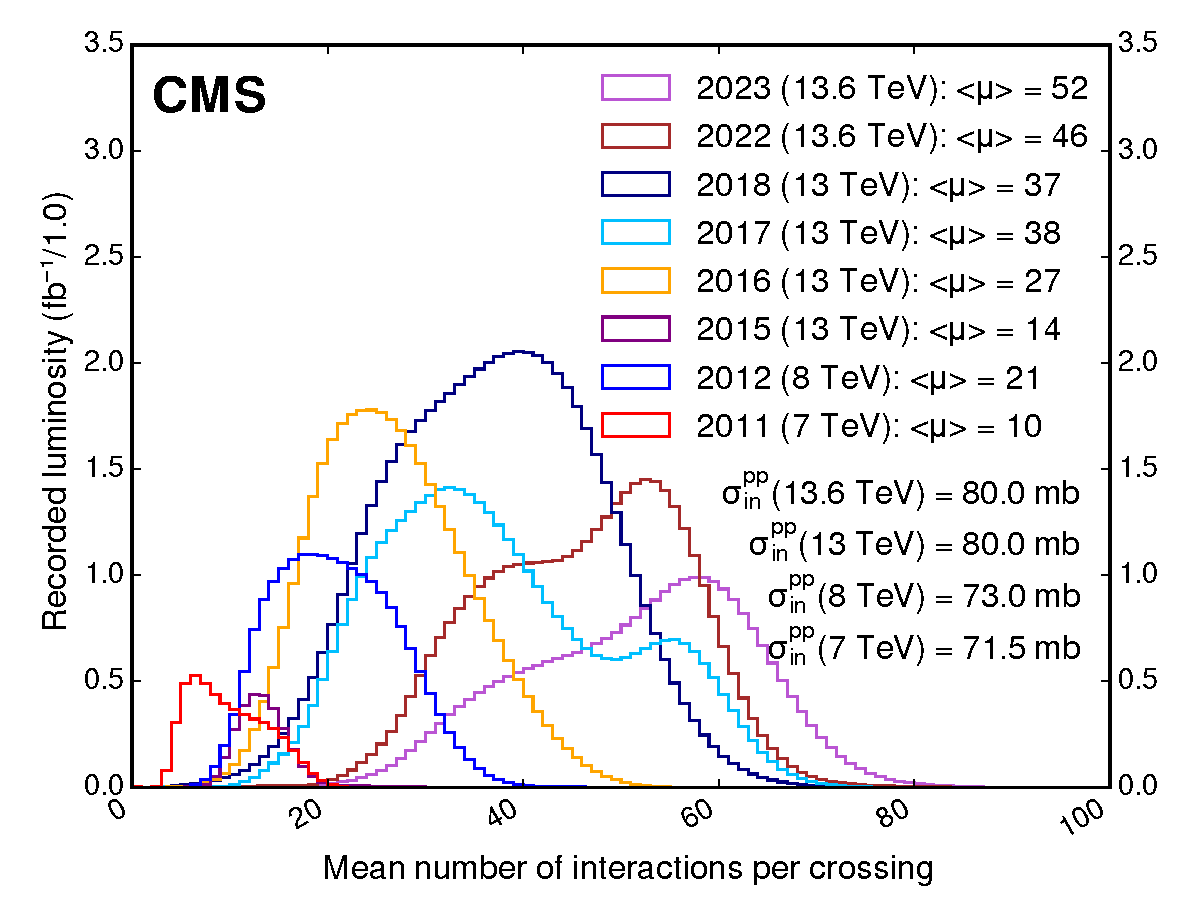
\includegraphics[width=0.8\linewidth]{figs/05_analysis/pileup_allYears.pdf}
	\caption[Pileup distributions and mean PU from 2011-2023 datataking~\cite{CMSlumi}]{Pileup distributions and mean PU from 2011-2023 datataking~\cite{CMSlumi}}
	\label{fig:pileup}
\end{figure}

Monte Carlo samples account for secondary collisions by generating PU interactions according to a predetermined distribution. However, this distribution does not exactly match what is observed in data. To account for this, we apply a weight to simulated samples as a function of the number of simulated PU interactions by dividing a histogram of data PU distributions by the Monte Carlo PU distribution.  %TODO: Make PU plots


\subsubsection{Monte Carlo Background} \label{sec:ana_mcbkg}
Although this analysis employs a data driven method of background estimation, simulated samples are used to inform on properties of background events and tune cuts to discriminate between signal and background. For this analysis, we use simulated Drell-Yan (DY) to $\ell\ell$ events with 0, 1 and 2 additional jets, simulated using matrix elements calculated at next-to-next-to leading order (NNLO). Studies were done with inclusive (any number of additional jets) samples but found to have worse agreement and statistical power compared to the jet categorized samples. The cross sections used for normalization were calculated using the \texttt{GenXSecAnalyzer}, a tool provided by CMS to calculate the cross sections for simulates samples~\cite{genxsecana}. A list of cross sections for each simulated process can be found in table~\ref{tab:mcsamples}.

\begin{table}[htb!]
	\centering
	\caption[List of simulated background processes and their cross sections calculated using \texttt{GenXSecAnalyzer}~\cite{genxsecana}]
	{List of simulated background processes and their cross sections calculated using \texttt{GenXSecAnalyzer}~\cite{genxsecana}}
	\label{tab:mcsamples}
	\begin{tabular}{l c}\hline
		Process & Cross Section [pb]\\
		\hline
		DY + 0 jets & 5090\\
		DY + 1 jet & 983.5\\
		DY + 2 jets & 353.5\\
		\hline
	\end{tabular}
	
\end{table}

\section{Vertex Reconstruction of Displaced Photon Pairs} \label{sec:ana_vertex}
\subsection{Diphoton Kinematics} \label{sec:vertex_calc}
The kinematics of a long lived scalar boson $\Phi$ decaying to two photons can be precisely described by the following
\begin{equation}\label{eq:me1e2theta}
	\text{m}_{\Phi}^2 = 2\text{E}_1\text{E}_2(1-\cos\theta)
\end{equation}
where the m$_\Phi$ is the mass of the $\Phi$, E$_1$ and E$_2$ are the energies of the two photons, and $\theta$ is the angle between the two photons. The energy of the two photons is measured by the CMS ECAL, thus $\theta$ can be calculated as a function of m$_\Phi$. Due to the primary vertex, decay vertex, and ECAL clusters being coplanar, this calculation is treated as a 2 dimensional problem. It is a trivial procedure to rotate the system to calculate the vertex, then rotate back to detector coordinates once the decay vertex is calculated. Let the position of the two ECAL clusters be \textbf{r$_1$} and \textbf{r$_2$}. The system can be rotated by an angle
\begin{equation} \label{eq:rot_angle}
	\varphi=\arccos\left(\frac{\textbf{r}_1\times\textbf{r}_2}{\|\textbf{r}_1\times\textbf{r}_2\|}\cdot\hat{z}\right)
\end{equation}
around an axis given by 
\begin{equation} \label{eq:rot_axis}
	\hat{n}=\frac{\textbf{r}_1\times\textbf{r}_2}{\|\textbf{r}_1\times\textbf{r}_2\|}\times\hat{z}
\end{equation}
to determine the decay vertex, then rotated by $-\varphi$ around the same axis to give the final value.

The geometry of the vertex fit is described in figure~\ref{fig:vertex_diagram}. Assume we have two ECAL clusters and a given value of m$_\Phi$. This fixes the value of $\theta$ from equation~\ref{eq:me1e2theta}. It will be shown that the locus of points satisfying these constraints corresponds to the arcs of a circle that overlaps the ECAL clusters.

\begin{figure}[htb]
	\centering
	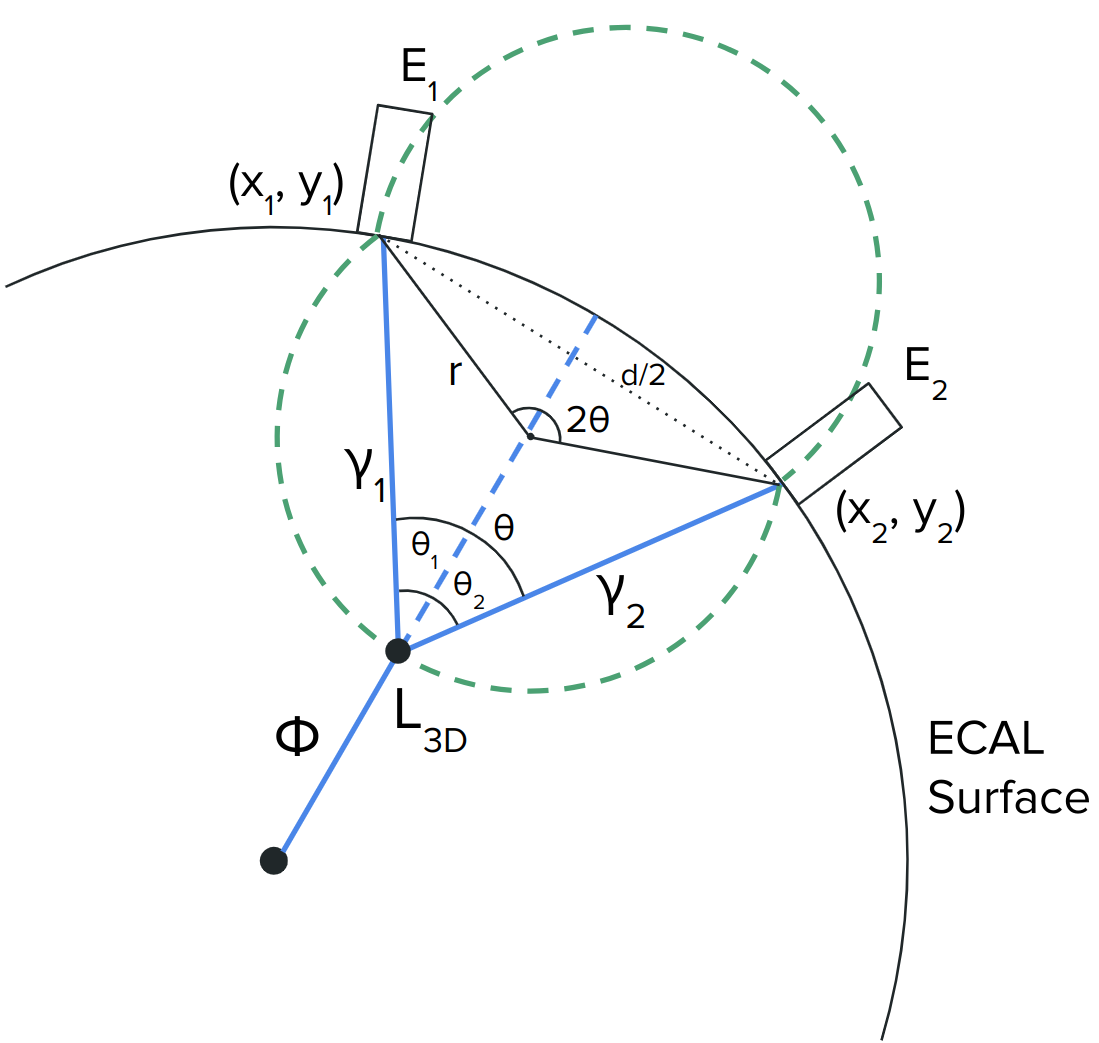
\includegraphics[width=0.65\linewidth]{figs/05_analysis/vertexfit_diagram.png}
	\caption{Geometrical configuration used to reconstruct the displaced vertex of the di-photon pair}
	\label{fig:vertex_diagram}
\end{figure}

Because three non-colinear points uniquely define a circle, $\theta$ corresponds to an inscribed angle on a circle which overlaps the decay vertex and the two ECAL clusters located at $(x_1, y_1)$ and $(x_2, y_2)$. The central angle of the arc between the two clusters has measure $2\theta$ by the inscribed angle theorem. From this, the radius of the circle can be defined by
\begin{equation} \label{eq:vertex_r}
	r=\frac{d}{2\sin{\theta}}
\end{equation}
where $d=\sqrt{(x_2-x_1)^2+(y_2-y_1)^2}$ is the distance between the two ECAL clusters. The center of the circle $(x_0, y_0)$ can be calculated by plugging the two ECAL cluster coordinates into the equation of a circle $(x-x_0)^2+(y-y_0)^2=r^2$, giving
\begin{equation} \label{eq:vertex_x0}
	x_0=\frac{x_1+x_2}{2}\pm\frac{y_1-y_2}{\text{q}}\cdot\sqrt{\text{r}^2-\frac{\text{q}^2}{4}}
\end{equation}
\begin{equation} \label{eq:vertex_y0}
	y_0=\frac{y_1+y_2}{2}\pm\frac{x_2-x_1}{\text{q}}\cdot\sqrt{\text{r}^2-\frac{\text{q}^2}{4}}
\end{equation}
\begin{equation} \label{eq:vertex_q}
	\text{where q}=\sqrt{(x_1-x_2)^2+(y_1-y_2)^2}
\end{equation}
The two solutions represent circles centered inside and outside of the ECAL. If $\theta<\pi/2$, then only the major arcs of the two circle satisfy equation~\ref{eq:me1e2theta}. Alternatively, if $\theta>\pi/2$ only the minor arcs are valid solutions. For either solution, an arc from one of two  circles will lie outside the ECAL. This arc represents a nonphysical solution and can be discarded, as it would imply the $\Phi$ both decayed outside of the ECAL and left ECAL clusters. The remaining arc represents the locus of possible decay vertices.

The angle between the two photons can be divided into the deflection of each photon ($\theta_1$ and $\theta_2$ respectively), and conservation of momentum requires $E_1\sin{\theta_1}-E_2\sin{\theta_2}=0$. From here, the vertex can be calculated numerically by sampling points along the remaining arc and choosing the coordinates that satisfy this equation.

It should be noted that this method can yield a locus of points that pass behind the beamline resulting in a negative impact parameter. The vertex is still calculated in these cases in order to provide a disjoint region with respect to the signal region that will be used to validate analysis methods and estimate the background yield. A diagram showing a negative reconstructed vertex is shown in figure~\ref{fig:negLxy}.

\begin{figure}[htb]
	\centering
	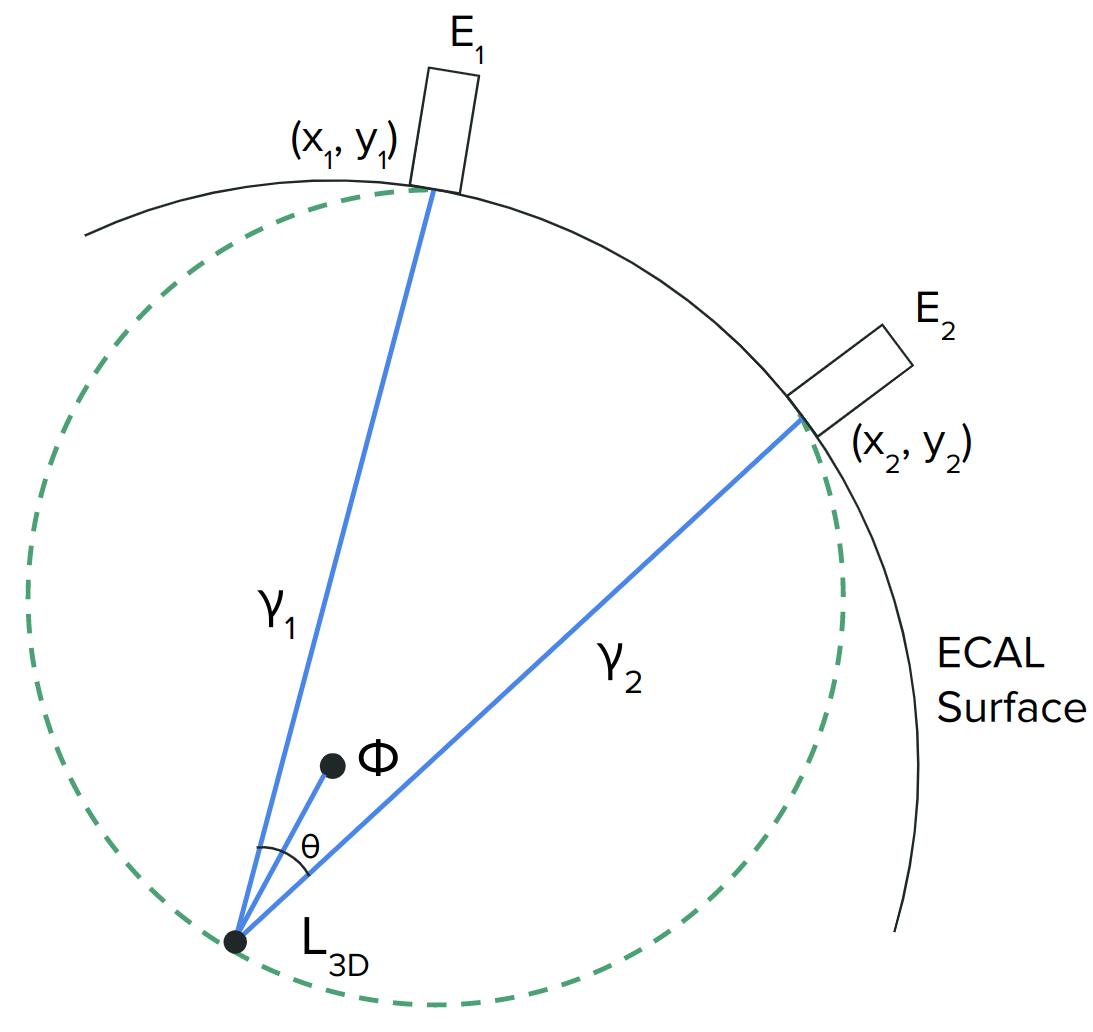
\includegraphics[width=0.65\linewidth]{figs/05_analysis/vertexfit_diagram_negativeLxy.png}
	\caption{Geometrical configuration showing the reconstruction of a negative impact parameter}
	\label{fig:negLxy}
\end{figure}

\subsection{Performance of Diphoton Vertex Calculation}\label{sec:ana_vertex_results}
It is evident that since the kinematic fit uses the hypothetical mass of the $\Phi$, the fit must be rerun for every hypothetical mass used in this analysis. As a result, the events in the signal region used for each value of $m_\Phi$ are different. Figure~\ref{fig:lxys_a} shows the reconstructed \lxy behaves as expected as the $\Phi$ lifetime increases. To demonstrate the resolution of the kinematic fit, we plot the difference between the calculated \lxy and the generator level \lxy as a function of the generator level \lxy, performed using a $\VZ\to\ell\ell$ samples with m$_\Phi=30\unit{GeV}$, using both the c$\tau=100\unit{mm}$ and $1000\unit{mm}$ samples. These distributions can be seen in figure~\ref{fig:lxys_b}. The vertical slices of this histogram were fit to Gaussian distributions so that the mean and sigma could be plotted as a function of generator level \lxy. The means shown in figure~\ref{fig:lxys_c} show the differences in calculated and generator \lxy are compatible with zero, and the sigma shown in figure~\ref{fig:lxys_d} show a resolution of $<3\unit{cm}$, slightly decreasing with generator level $\lxy$. Both the mean and sigma remain consistent across all ranges of m$_\Phi$.

\begin{figure}[htb!]
	\centering
	\captionsetup[subfigure]{justification=centering}
	\begin{subfigure}[h]{0.45\linewidth}
		\centering
		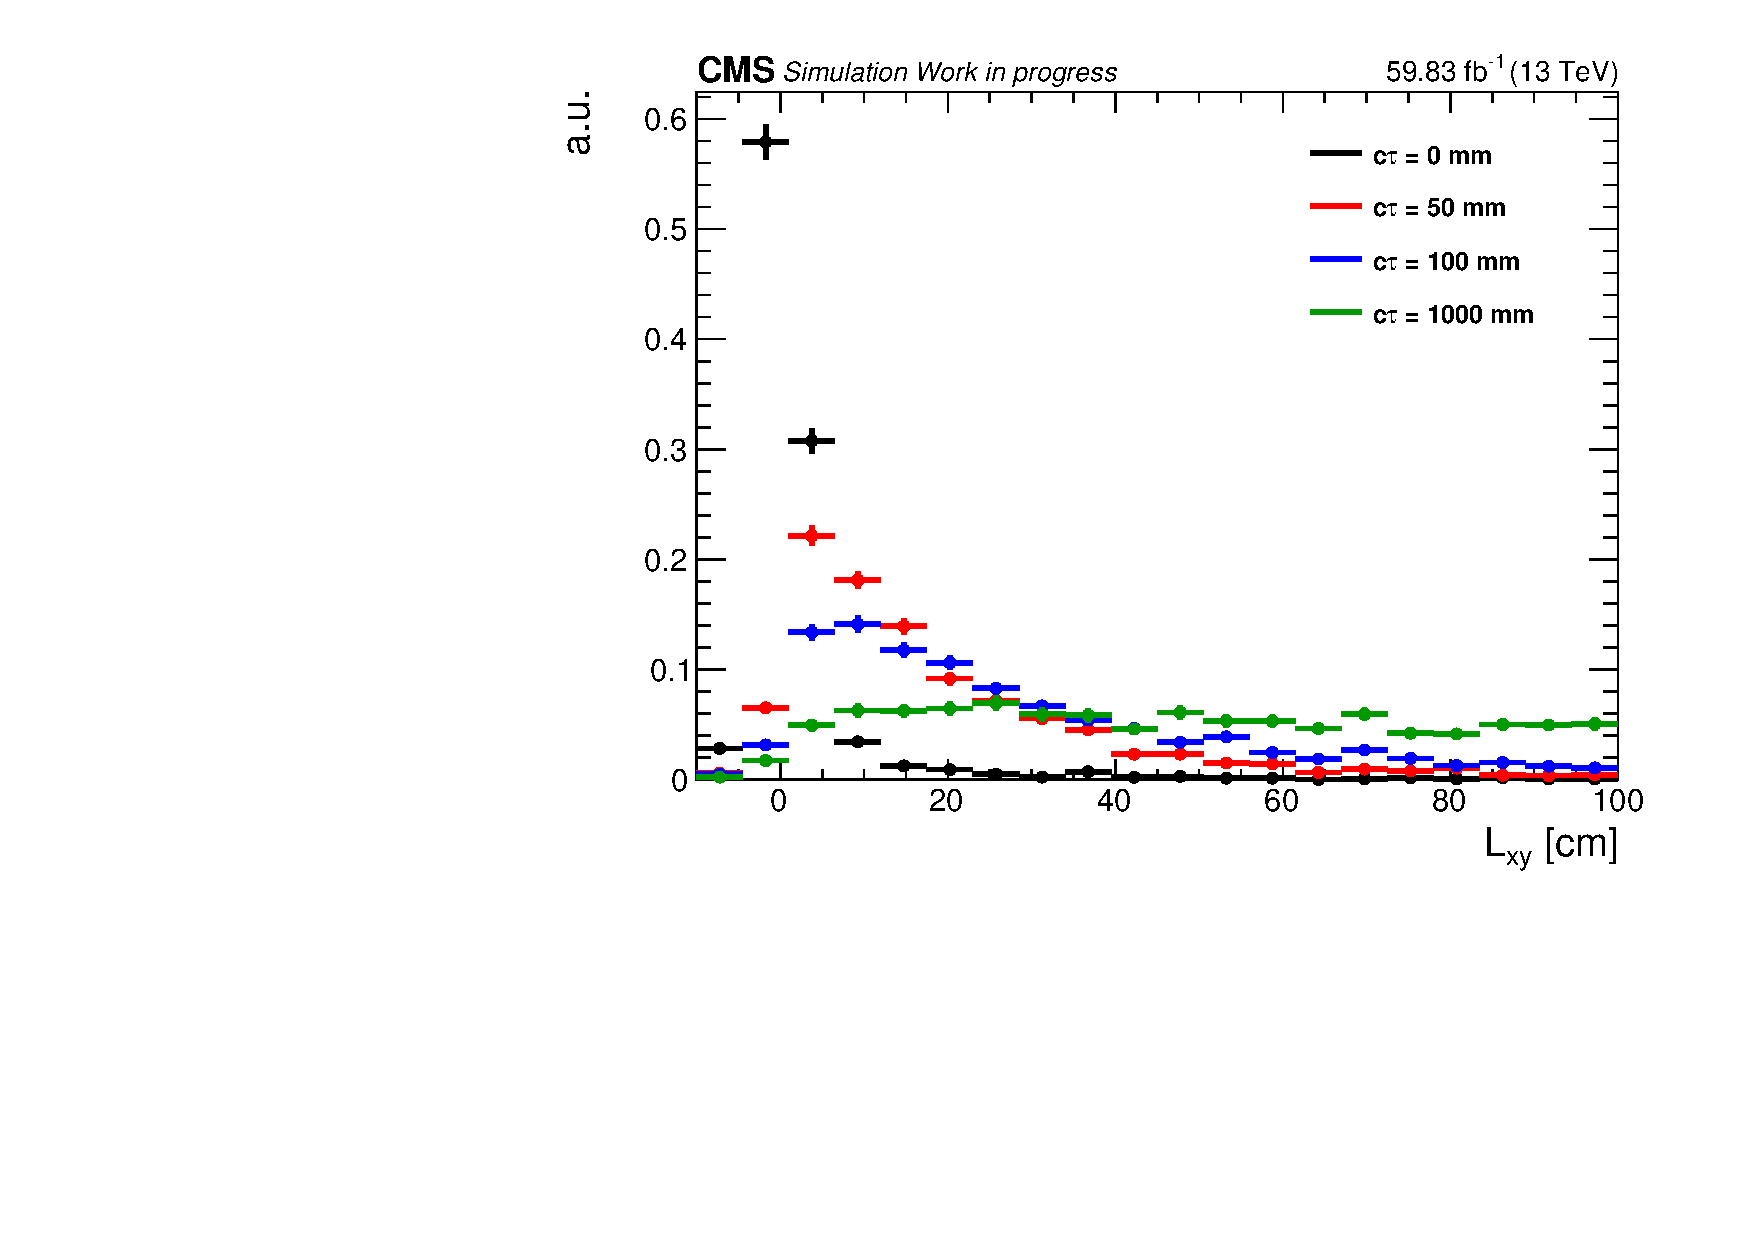
\includegraphics[width=\linewidth]{figs/05_analysis/2018_signalLxy_comparison.pdf}
		\caption{\lxy distribution calculated for $m_\Phi=30\unit{GeV}$, $\VZ\to\ell\ell$ signal samples}
		\label{fig:lxys_a}
	\end{subfigure}
	\begin{subfigure}[h]{0.45\linewidth}
		\centering
		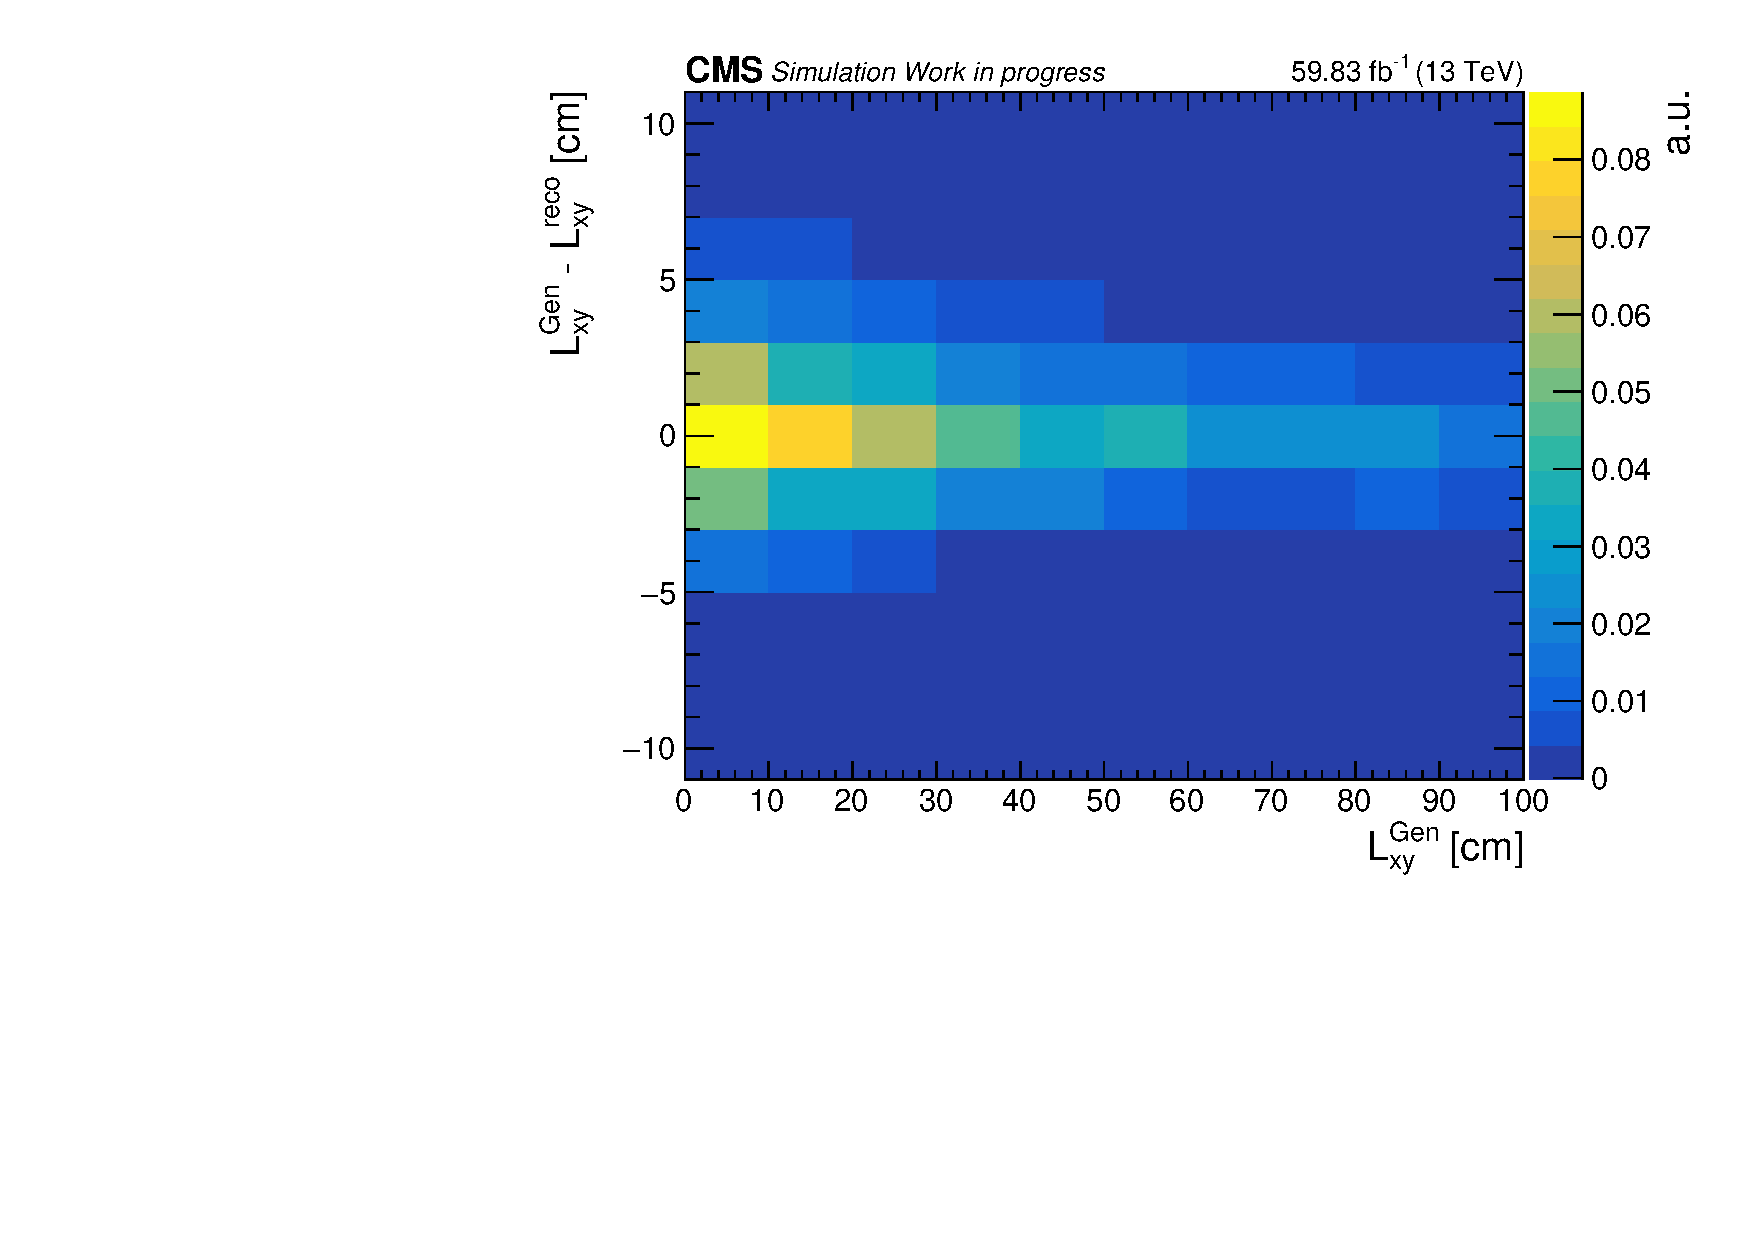
\includegraphics[width=\linewidth]{figs/05_analysis/2018_deltaLxyVsLxy_Z_m30.pdf}
		\caption{The $\Delta\lxy$ vs $\lxy$ distributions for signal events with exactly 2 photons}
		\label{fig:lxys_b}
	\end{subfigure}
	\begin{subfigure}[h]{0.45\linewidth}
		\centering
		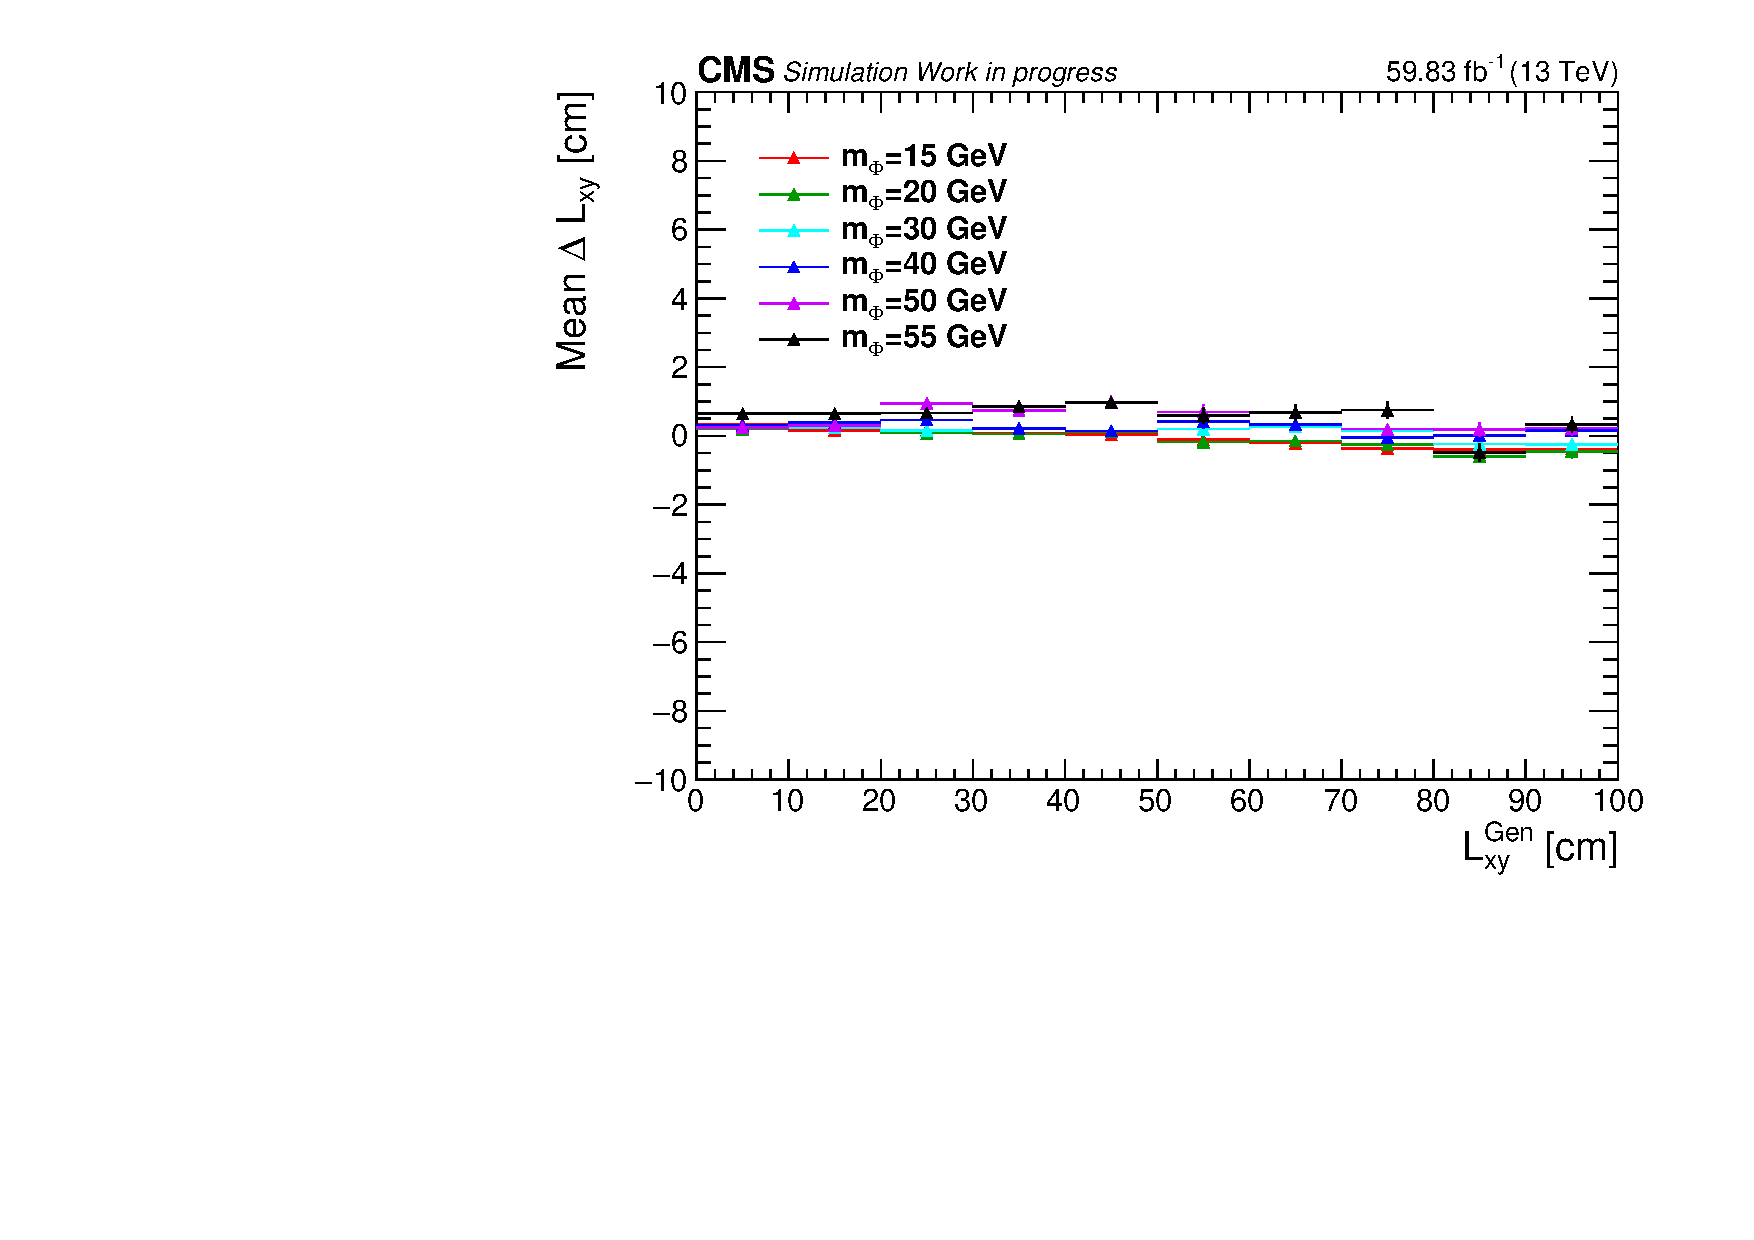
\includegraphics[width=\linewidth]{figs/05_analysis/2018_meanLxyVsLxy_Z_all.pdf}
		\caption{Mean of Gaussian slice fits}
		\label{fig:lxys_c}
	\end{subfigure}
	\begin{subfigure}[h]{0.45\linewidth}
		\centering
		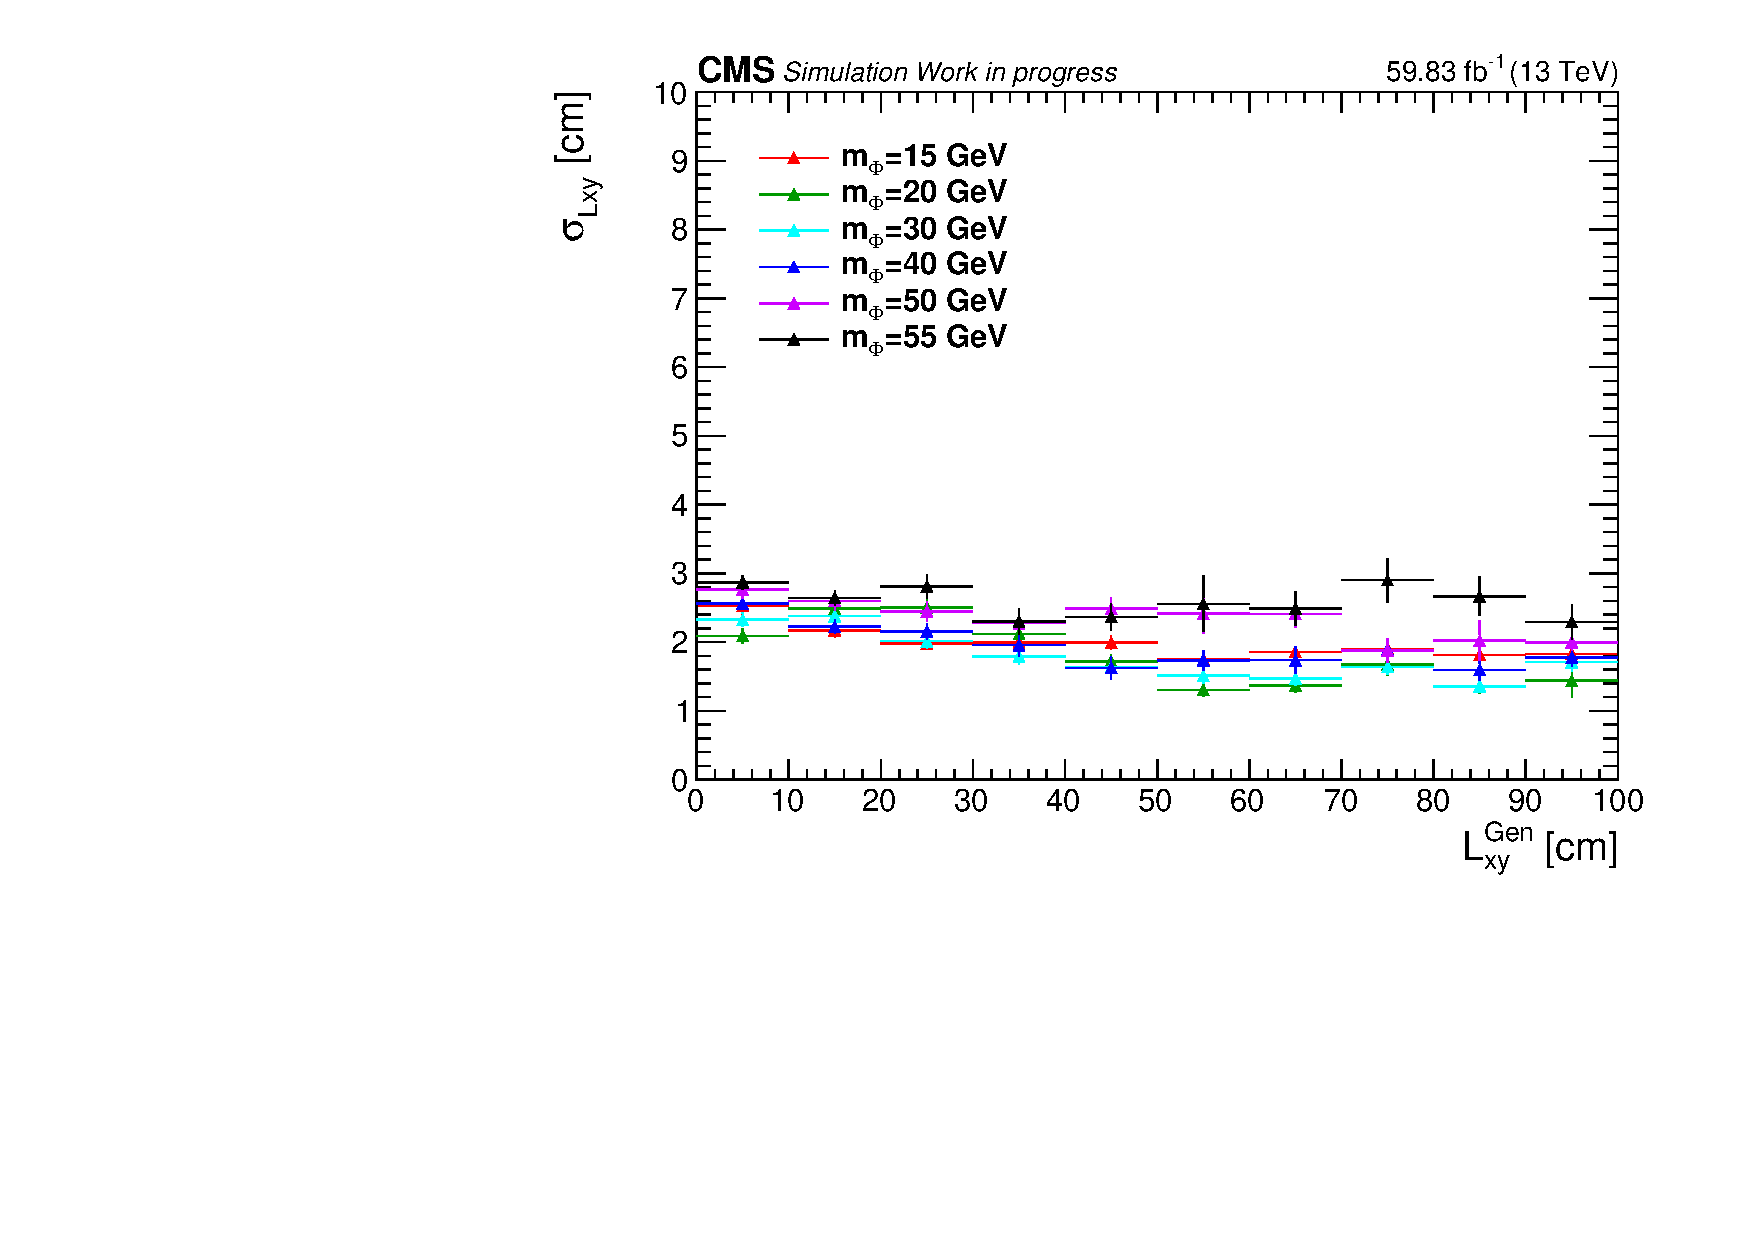
\includegraphics[width=\linewidth]{figs/05_analysis/2018_sigmaLxyVsLxy_Z_all.pdf}
		\caption{Sigma of Gaussian slice fits}
		\label{fig:lxys_d}
	\end{subfigure}
	\caption[Performance of the vertex calculation on signal samples. The fit shows good agreement across all values of generator level \lxy and a resolution of $<3\unit{cm}$.]{Performance of the vertex calculation on signal samples. The fit shows good agreement across all values of generator level \lxy and a resolution of $<3\unit{cm}$.}
	\label{fig:lxys}
\end{figure}

It can be shown that the calculated \lxy for an assumed value of \mphi is monotonically decreasing with the prompt invariant diphoton mass \mgg. Assume that two photons have a prompt invariant mass \mgg. Calculating the vertex assuming $\mphi=\mgg$ would yield a vertex with $\lxy=0$ by construction. Calculating the vertex assuming $\mphi>\mgg$ would cause the angle between the two photons given by equation~\ref{eq:me1e2theta} to decrease. As the ECAL cluster positions are fixed, this pushes the vertex backwards yielding $\lxy<0$. By similar methods, assuming a value of $\mphi<\mgg$ yields a vertex with $\lxy>0$. The dependence makes the \lxy very sensitive to small changes in the assumed value of \mphi. If the assumed value of \mphi differs from the true mass by $5\unit{GeV}$, the calculated \lxy can skew upwards or downwards by $>20\unit{cm}$, depending on the value of the true mass. Figure~\ref{fig:deltaLxy} shows the differences in generated and reconstructed \lxy, combining samples for all lifetimes for a given true mass.

\begin{figure}[htb!]
	\centering
	\captionsetup[subfigure]{justification=centering}
	\begin{subfigure}[h]{0.45\linewidth}
		\centering
		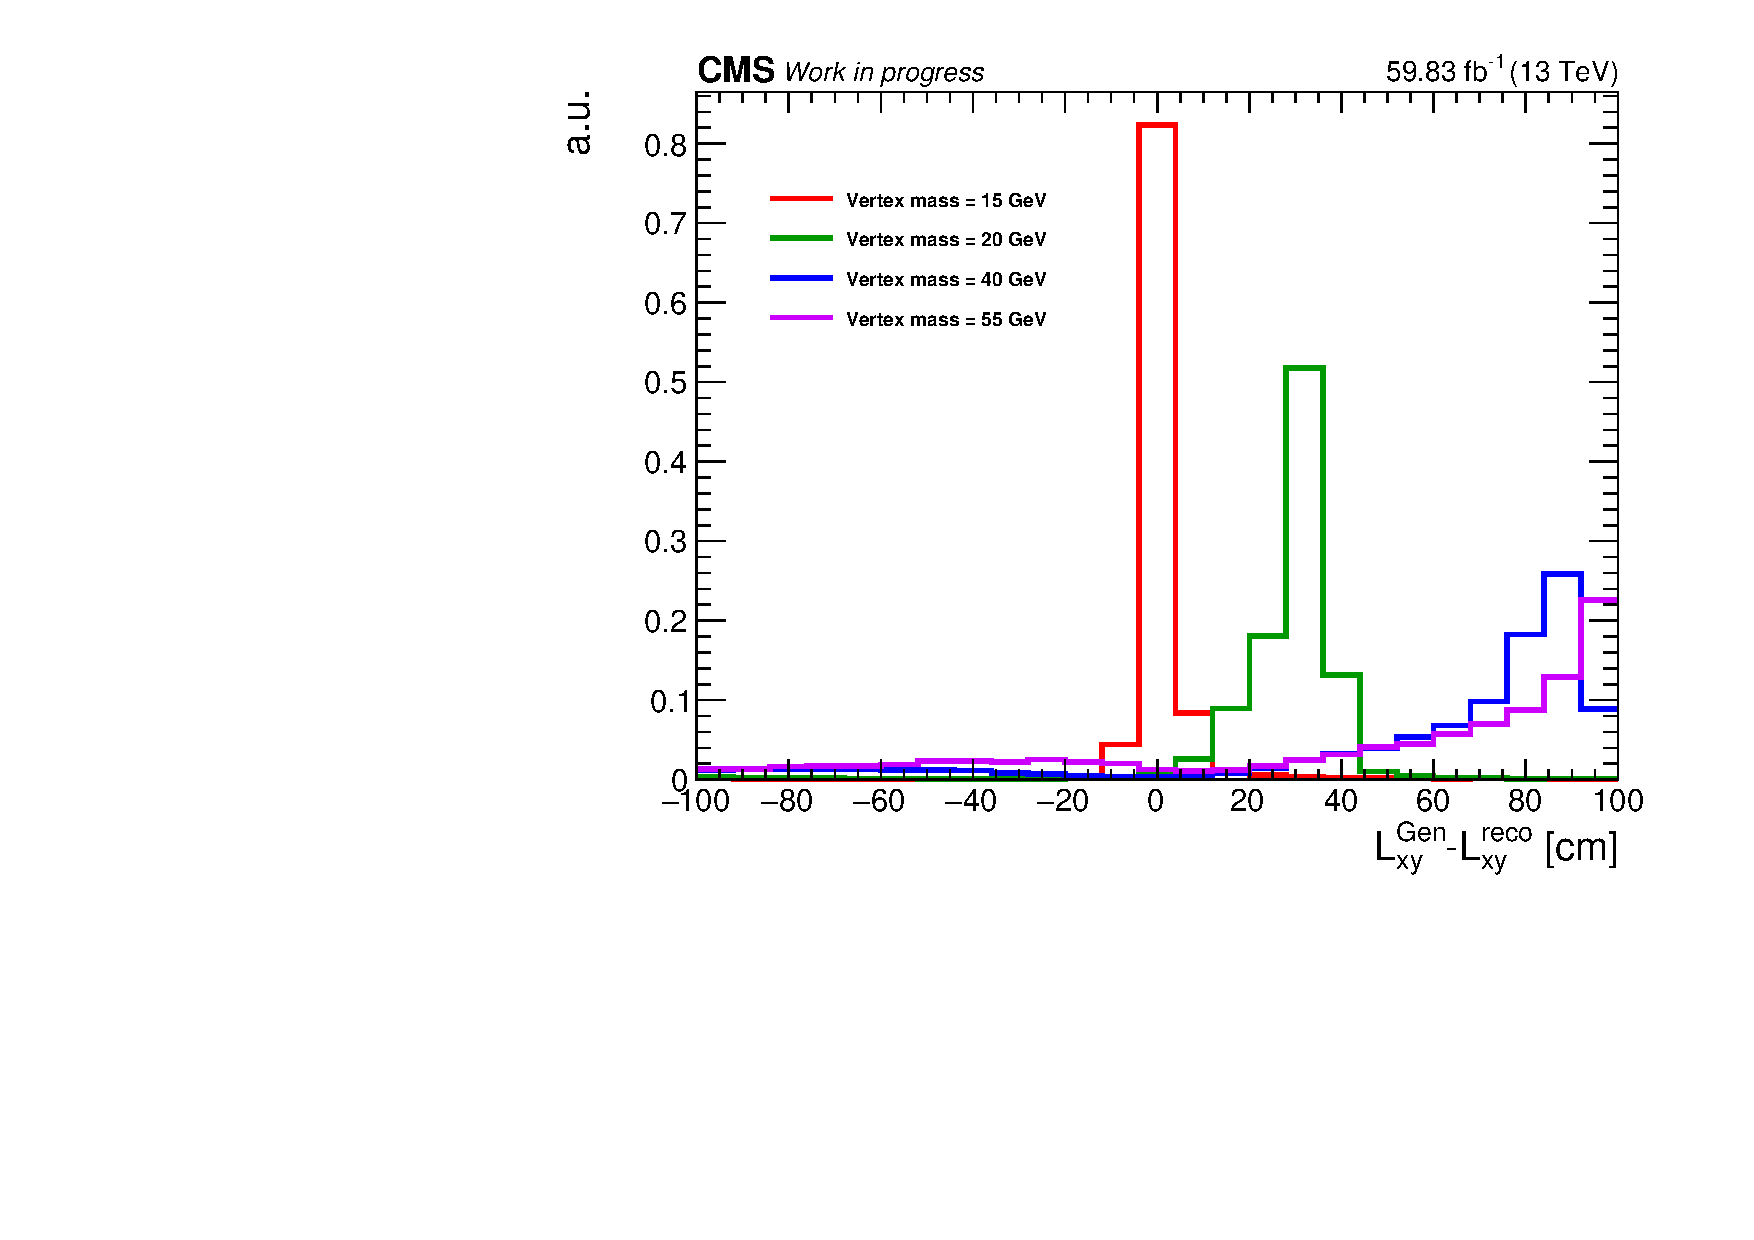
\includegraphics[width=\linewidth]{figs/05_analysis/2018_deltaLxy_Z_m15.pdf}
		\caption{$\mphi=15\unit{GeV}$}
	\end{subfigure}
	\begin{subfigure}[h]{0.45\linewidth}
		\centering
		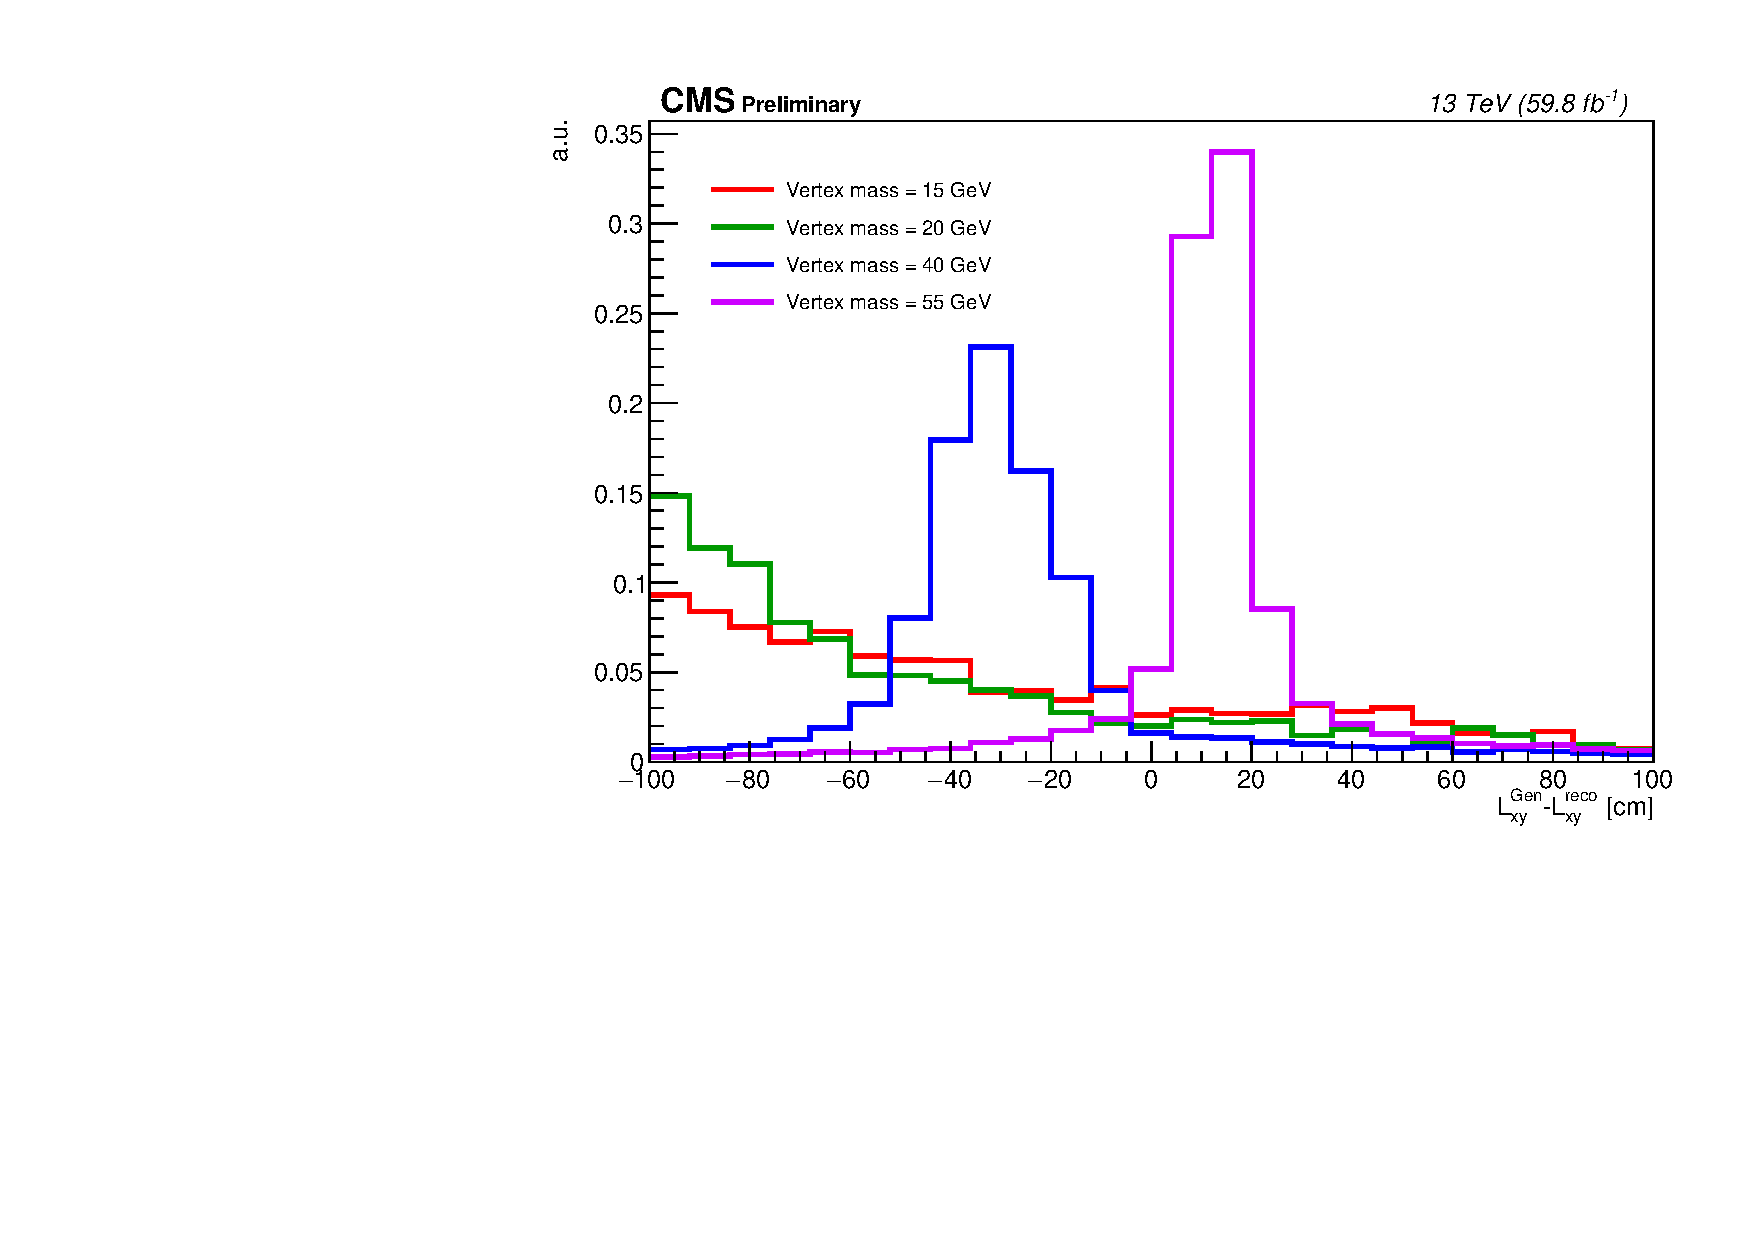
\includegraphics[width=\linewidth]{figs/05_analysis/2018_deltaLxy_Z_m50.pdf}
		\caption{$\mphi=50\unit{GeV}$}
	\end{subfigure}
	\caption[The difference between the true and reconstructed vertex grows as the assumed mass departs from the true one. Gen-reconstructed $\lxy$ for a \VZ+\VH samples under several assumed mass points.]{The difference between the true and reconstructed vertex grows as the assumed mass departs from the true one. Gen-reconstructed $\lxy$ for a \VZ+\VH samples under several assumed mass points.}
	\label{fig:deltaLxy}
\end{figure}

This analysis uses the \texttt{nanoAODv9} data format - the most compact data tier available for analysis use in CMS. As opposed to lower tier formats which contain detailed collections of classes to store event properties, nanoAOD provides only the most important information for high level physics objects~\cite{nanoaod}. This information includes several properties of photons but omits the calorimeter cluster position, which is required to calculate the diphoton vertex. To circumvent this, we propagate the photons from the PV to the ECAL using their $\eta$ and $\phi$. The ECAL is approximated using a cylinder with radius $\rho=137\unit{cm}$ and $z=324\unit{cm}$. These values were obtained using \texttt{miniAODv2} samples and are shown in figure~\ref{fig:calo_position}. Diphoton vertices calculated using the propagated coordinates yield a \lxy within 3\% of the \lxy calculations using the exact cluster coordinates, which is well within the intrinsic resolution of the vertex calculation.

\begin{figure}[htb!]
	\centering
	\captionsetup[subfigure]{justification=centering}
	\begin{subfigure}[h]{0.45\linewidth}
		\centering
		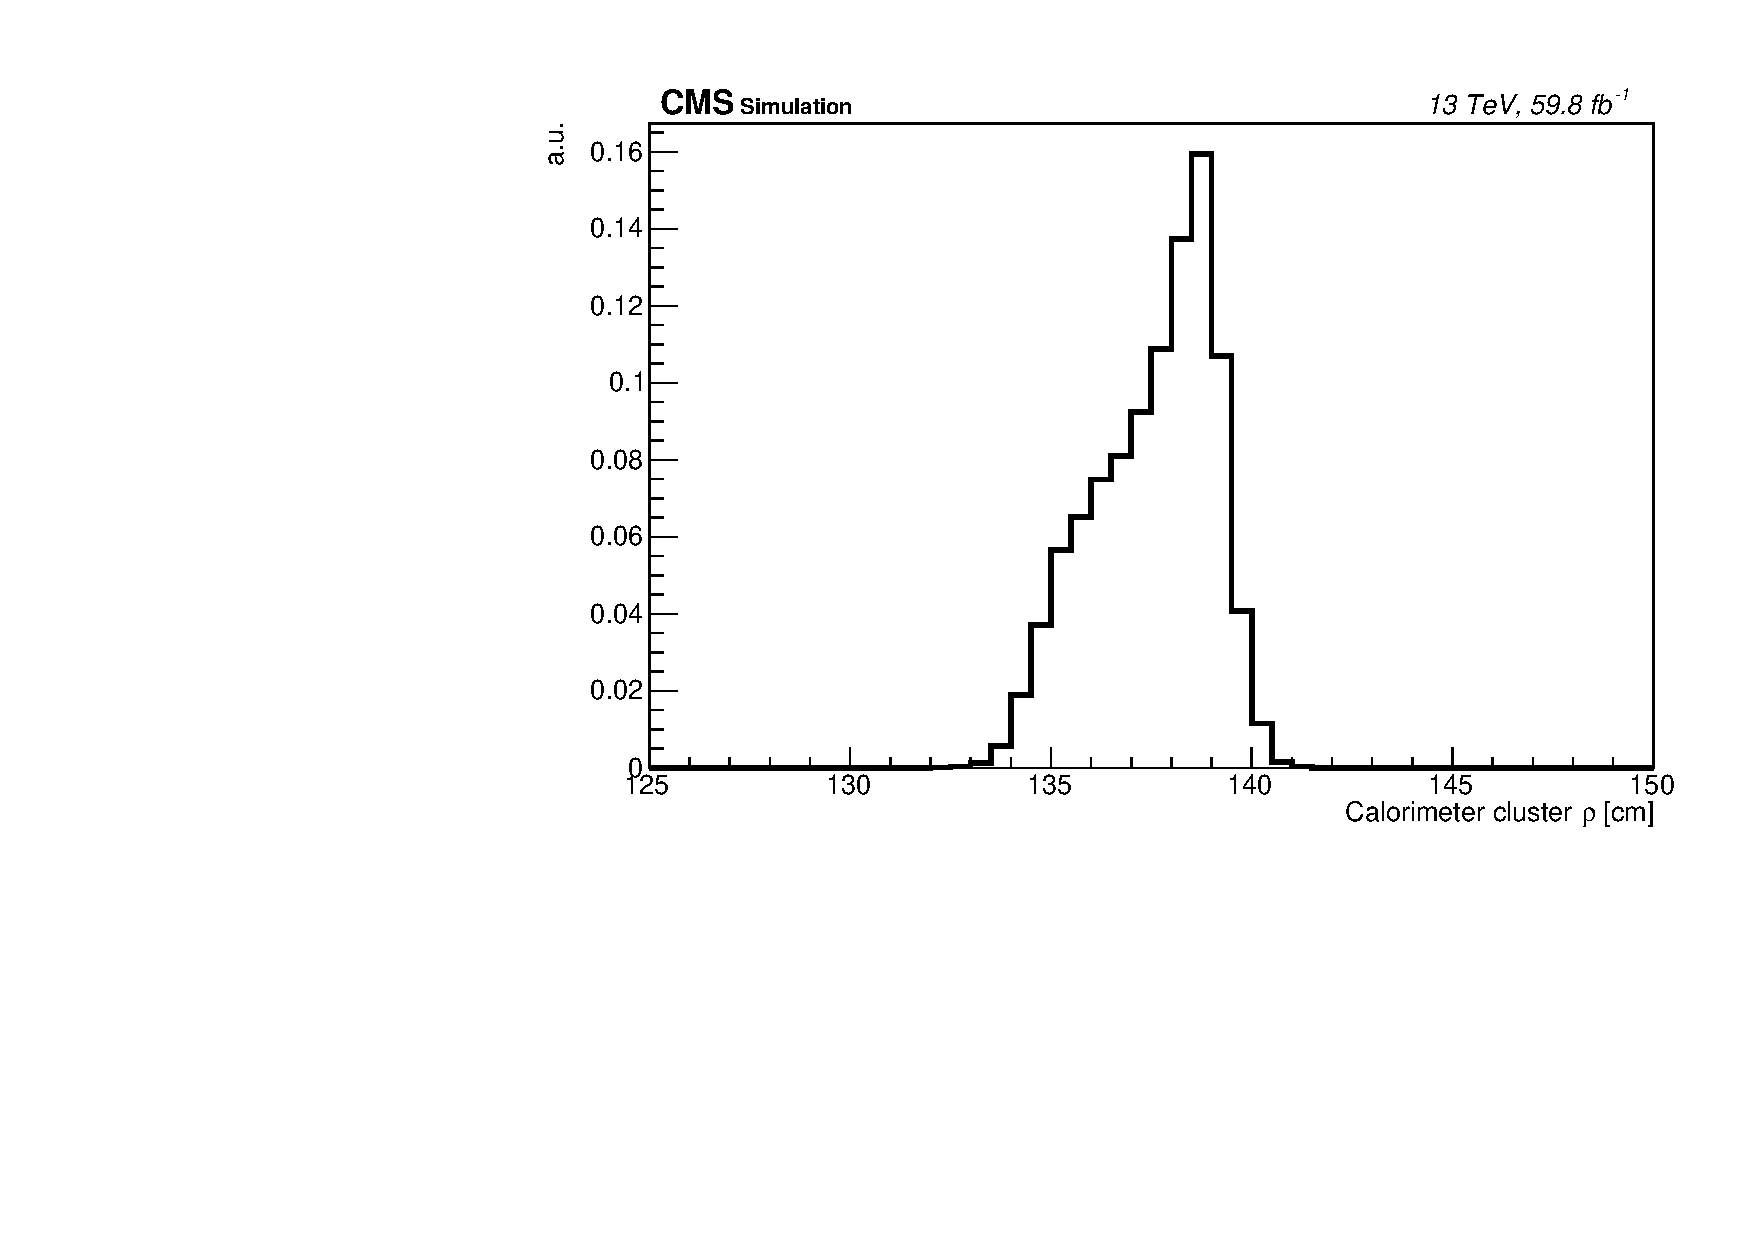
\includegraphics[width=\linewidth]{figs/05_analysis/calorimeter_rho.pdf}
		\caption{Calormieter cluster $\rho$}
	\end{subfigure}
	\begin{subfigure}[h]{0.45\linewidth}
		\centering
		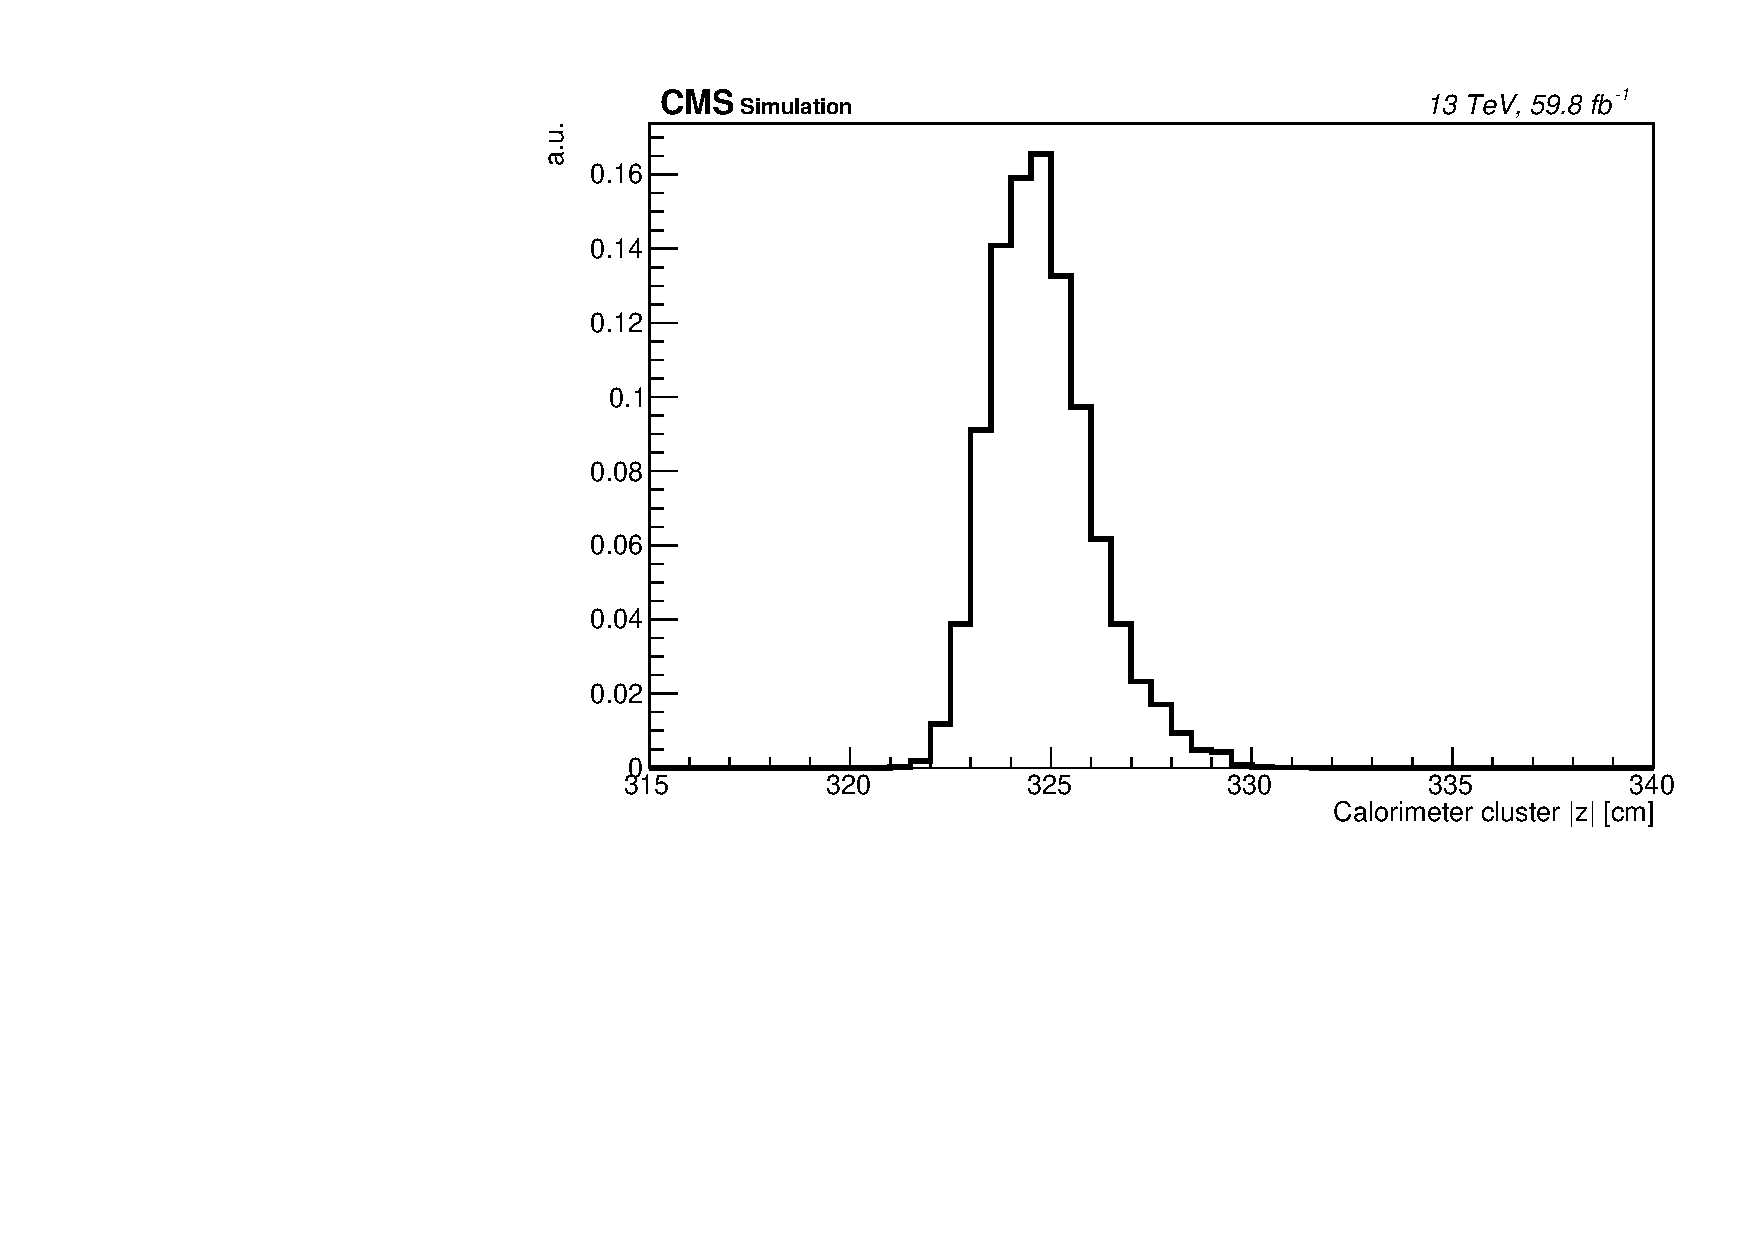
\includegraphics[width=\linewidth]{figs/05_analysis/calorimeter_z.pdf}
		\caption{Calorimeter cluster $|z|$}
	\end{subfigure}
	\caption{The $\rho$ for barrel photons and $|z|$ for endcap photons for all reconstructed photons using \texttt{miniAODv2} signal samples}
	\label{fig:calo_position}
\end{figure}

\section{Event Selection} \label{sec:ana_eventsel}
The first step in collecting events for the analysis is to select events passing HLT lepton triggers. Events passing these triggers are then chosen based on the presence of two same flavor, opposite charge leptons and two photons. Various quality cuts, referred to as preselection criteria, are applied to these objects to reject background. Lastly, cuts are applied to reject photons from final state radiation (FSR) and low \pt photons that promoted to displaced $\Phi$ candidates by the kinematic vertex fit.

\subsection{Triggers} \label{sec:ana_triggers}
Events are triggered through leptonic decays of the \VZ boson produced in association with the SM Higgs Boson. The \VZ candidates are selected from dilepton events passing the HLT isolated single lepton triggers. These triggers are the standard lepton triggers recommended both the EGamma and Muon physics object groups (POGs) in CMS. Double lepton and high \pt lepton triggers were considered but provide only negligible improvement when applied in addition to the single lepton triggers. Muon events must pass the single muon triggers and are vetoed by the single electron triggers, while electron events must pass single electron triggers and are vetoed by the single muon triggers. A complete list of HLT trigger paths used for each year can be see in table~\ref{tab:triggers}.

\begin{table}[h]
	\caption[HLT trigger paths used for the Run 2 datasets]{HLT trigger paths used for the Run 2 datasets} 
	\label{tab:triggers}
	\begin{center}
		\begin{tabular}{l|l|l}\hline
			Year & Single Electron & Single Muon\\
			\hline
			2018 & HLT\_Ele32\_WPTight\_Gsf & HLT\_IsoMu24\\
			2017 & HLT\_Ele32\_WPTight\_Gsf & HLT\_IsoMu27\\
			2016 & HLT\_Ele27\_WPTight\_Gsf & HLT\_IsoMu24 \textbar\textbar HLT\_IsoTkMu24\\
			\hline
		\end{tabular}
	\end{center}
\end{table}

\subsection{Preselection Criteria} \label{sec:ana_preselection}
For both electrons and muons we define a set of tight and loose leptons based on cut based ID set by the EGamma and Muon POGs. To reconstruct a \VZ candidate, we require exactly two same flavor opposite charge tight leptons with invariant mass $70<m_{\ell\ell}<110\unit{GeV}$ and zero additional loose leptons. For photons we require two photons passing a set of preselection criteria, which are subject to additional classification based on cut based ID.

\subsubsection{Particle Flow Isolation} \label{sec:ana_isolation}
One key application of the particle flow (PF) algorithm is the calculation of a particle's isolation. This quantity measures the \pt contributions from PF candidates in a fixed $\Delta R$ cone centered on the original particle. A lower value implies the particle is more isolated (i.e. there are fewer additional particles nearby), and vice versa. Isolation is a key variable to reject particles produced in jets from heavy-flavor hadronic decays or decays of pions and kaons~\cite{Sirunyan:PF}. A particle's isolation is defined as follows:
\begin{equation}
	\label{eq:pfiso}
	I_\text{pf} = \sum_{\substack{i\in\text{charged}\\\text{hadrons}}}^{\Delta R}\pt^i+\text{max}\left(0,\sum_{\substack{i\in\text{neutral}\\\text{hadrons}}}^{\Delta R}\et^i+\sum_{\gamma\in\text{photons}}^{\Delta R}\et^\gamma-\text{PU Corrections}\right)
\end{equation}
Particles created from pileup can create calorimeter deposits within the $\Delta R$ cone used to calculate isolation. These are unrelated to the physics process for the central particle and can artificially inflate the isolation of a particle. Only charged hadrons originating from the PV are used when calculating the charged hadron isolation, which rejects charged hadrons originating from PU. Neutral particles, however, do not produce tracks, meaning calorimeter deposits from the PV and from pileup are indistinguishable. Because of this, there are additional corrections for the neutral hadron and photon isolation. Two common methods are $\rho$ corrections, which calculate the average energy density from pileup multiplied by an effective area as a function of $\eta$, and $\delta\beta$ corrections, which calculate the energy from pileup as a function of the charged hadron contribution from PU.

It is also common to refer to a particle's relative isolation, which is defined as
\begin{equation}
	\label{eq:reliso}
	I_\text{rel}=\frac{I_\text{pf}}{\pt}
\end{equation}

\subsubsection{Muon Criteria} \label{sec:ana_muons}
The NanoAOD data format takes reconstructed muons and applies loose cuts before storing the muon properties. These branches contain all muons with $\pt>3\unit{GeV}$ with minimal cuts to reconstruction quality. For the purpose of this analysis, muons are classified as loose if they pass all of the following criteria:
\begin{itemize}
	\item $\pt>10\unit{GeV}$
	\item $|\eta|<2.4$
	\item $D_{xy}<0.2\unit{cm}$: the transverse distance from the PV to the beamline must be less than 0.2 cm
	\item $D_{z}<0.5\unit{cm}$: the longitudinal distance from the PV to the beamline must be less than 0.5 cm
	\item $I_\text{rel}(\Delta R<0.4,\,\delta\beta\text{-corrected})<0.25$
	\item Passes loose quality criteria set by the Muon POG
	\begin{itemize}
		\item Muon must be reconstructed by the PF algorithm
		\item Muon must be either a global and/or tracker muon
	\end{itemize}
\end{itemize}
We define tight muons as a subset of loose muons if they pass the following criteria:
\begin{itemize}
	\item $I_\text{rel}(\Delta R<0.4,\,\delta\beta\text{-corrected})<0.15$
	\item Passes tight quality criteria set by the Muon POG
	\begin{itemize}
		\item Muon must be a global muon
		\item The global muon track fit must have $\chi^2/\text{ndof}<10$
		\item Global track must have at least one hit in a muon chamber %TODO: why is this necessary if it's already a global muon?
		\item Muon track must have segments in at least 2 different muon stations %TODO: same question
		\item Tracker track $D_{xy}<2\unit{mm}$
		\item Tracker track $D_{z}<5\unit{mm}$
		\item Tracker track must have at least 1 hit in the pixel detector
		\item Tracker track must have hits in more than 5 tracker layers
	\end{itemize}
\end{itemize}
We also require that one of the two tight muons used to reconstruct the \VZ to be the triggering muon, and that the triggering muon have $\pt>25\unit{GeV}$ ($28\unit{GeV}$ in 2017) in order to operate above the single muon trigger thresholds.

\subsubsection{Electron Criteria} \label{sec:ana_electrons}
Analogously to the muon criteria, loose electrons are defined from reconstructed global event description electrons if they pass a set of preselection criteria. 
\begin{itemize}
	\item $\pt>15\unit{GeV}$
	\item $|\eta|<2.4$
	\item $|\eta|>1.57\ \ \textbar\textbar\ \ |\eta|<1.44$: rejects photons in the overlap region between the ECAL barrel and endcap
	\item $D_{xy}<0.2\unit{cm}$, $D_{z}<0.2\unit{cm}$
	\item Passes cut based ID provided by the EGamma POG at the \texttt{veto} working point
\end{itemize}
Tight electrons are selected from this collection of they pass cut based ID at the \texttt{tight} working point. Similar to the muon criteria, we require one of the tight electrons be the triggering electron, and that the triggering electron have $\pt>35\unit{GeV}$.

The variables used in the cut based ID have different working points for barrel and endcap electrons and are optimized to reject background such as photons in hadronic showers or converted photons. The spread of the calorimeter cluster is measured using $\sigma_{i\eta i\eta}$, which is the covariance of the cluster shape measured in a $5\times5$ grid of calorimeter crystals. Clusters from signal electrons are exp The $H/E$ ratio takes the energy of HCAL clusters located behind the ECAL cluster and divides it by the ECAL cluster energy. Clusters created from EM showers are expected to have relatively narrower shower shape and deposit less energy in the HCAL than hadronic showers, so these two variables are strong handles to reject hadronic background. Tracker information is also used to separate signal from background. The $|\Delta\eta_\text{seed}|$ and $|\Delta\phi_\text{in}|$ are the difference in track $\eta$/$\phi$ and supercluster $\eta$/$\phi$. A complete table of cut values for these variables can be seen in tables~\ref{tab:electron_barrel},\ref{tab:electron_endcap}. 

\begin{table}[htb!]
	\centering
	\caption[Cut based ID selection criteria for barrel electrons in Run-2~\cite{electronid}]{Cut based ID selection criteria for barrel electrons in Run-2~\cite{electronid}}
	\label{tab:electron_barrel}
	\begin{tabular}{l | r | r}
		\hline
		& Veto & Tight \\
		\hline
		\hline
		$\sigma_{i\eta i\eta}<$ & 0.0126 & 0.0104 \\
		$|\Delta\eta_\text{seed}|<$ & 0.0463 & 0.00255 \\
		$|\Delta\phi_\text{In}|<$ & 0.148 & 0.022 \\
		$H/E<$ & $0.05+1.16/E+0.0324\rho/E$ & $0.026+1.15/E+0.0324\rho/E$ \\
		$I_\text{rel}(\rho\text{-area corrected})<$ & $0.198+0.506/\pt$ & $0.0287+0.506/\pt$\\
		$|1/E-1/p|<$  & 0.209 & 0.159 \\
		Missing inner hits $\leq$ & 2 & 1 \\
		Passes conversion veto & True & True\\
		\hline
	\end{tabular}
\end{table}

\begin{table}[htb!]
	\centering
	\caption[Cut based ID selection criteria for endcap electrons in Run-2~\cite{electronid}]{Cut based ID selection criteria for endcap electrons in Run-2~\cite{electronid}}
	\label{tab:electron_endcap}
	\begin{tabular}{l | r | r}
		\hline
		& Veto & Tight \\
		\hline
		\hline
		$\sigma_{i\eta i\eta}<$ & 0.0457 & 0.0353 \\
		$|\Delta\eta_\text{seed}|<$ & 0.00814 & 0.00501 \\
		$|\Delta\phi_\text{In}|<$ & 0.19 & 0.0236 \\
		$H/E<$ & $0.05+2.54/E+0.183\rho/E$ & $0.0188+2.06/E+0.183\rho/E$ \\
		$I_\text{rel}(\rho\text{-area corrected})<$ & $0.203+0.963/\pt$ & $0.0445+0.963/\pt$\\
		$|1/E-1/p|<$ & 0.132 & 0.0197 \\
		Missing inner hits $\leq$= & 3 & 1 \\
		Passes conversion veto & True & True\\
		\hline
	\end{tabular}
\end{table}
